% Options for packages loaded elsewhere
\PassOptionsToPackage{unicode}{hyperref}
\PassOptionsToPackage{hyphens}{url}
\PassOptionsToPackage{dvipsnames,svgnames,x11names}{xcolor}
%
\documentclass[
  letterpaper,
  DIV=11,
  numbers=noendperiod]{scrartcl}

\usepackage{amsmath,amssymb}
\usepackage{iftex}
\ifPDFTeX
  \usepackage[T1]{fontenc}
  \usepackage[utf8]{inputenc}
  \usepackage{textcomp} % provide euro and other symbols
\else % if luatex or xetex
  \usepackage{unicode-math}
  \defaultfontfeatures{Scale=MatchLowercase}
  \defaultfontfeatures[\rmfamily]{Ligatures=TeX,Scale=1}
\fi
\usepackage{lmodern}
\ifPDFTeX\else  
    % xetex/luatex font selection
\fi
% Use upquote if available, for straight quotes in verbatim environments
\IfFileExists{upquote.sty}{\usepackage{upquote}}{}
\IfFileExists{microtype.sty}{% use microtype if available
  \usepackage[]{microtype}
  \UseMicrotypeSet[protrusion]{basicmath} % disable protrusion for tt fonts
}{}
\makeatletter
\@ifundefined{KOMAClassName}{% if non-KOMA class
  \IfFileExists{parskip.sty}{%
    \usepackage{parskip}
  }{% else
    \setlength{\parindent}{0pt}
    \setlength{\parskip}{6pt plus 2pt minus 1pt}}
}{% if KOMA class
  \KOMAoptions{parskip=half}}
\makeatother
\usepackage{xcolor}
\setlength{\emergencystretch}{3em} % prevent overfull lines
\setcounter{secnumdepth}{-\maxdimen} % remove section numbering
% Make \paragraph and \subparagraph free-standing
\ifx\paragraph\undefined\else
  \let\oldparagraph\paragraph
  \renewcommand{\paragraph}[1]{\oldparagraph{#1}\mbox{}}
\fi
\ifx\subparagraph\undefined\else
  \let\oldsubparagraph\subparagraph
  \renewcommand{\subparagraph}[1]{\oldsubparagraph{#1}\mbox{}}
\fi


\providecommand{\tightlist}{%
  \setlength{\itemsep}{0pt}\setlength{\parskip}{0pt}}\usepackage{longtable,booktabs,array}
\usepackage{calc} % for calculating minipage widths
% Correct order of tables after \paragraph or \subparagraph
\usepackage{etoolbox}
\makeatletter
\patchcmd\longtable{\par}{\if@noskipsec\mbox{}\fi\par}{}{}
\makeatother
% Allow footnotes in longtable head/foot
\IfFileExists{footnotehyper.sty}{\usepackage{footnotehyper}}{\usepackage{footnote}}
\makesavenoteenv{longtable}
\usepackage{graphicx}
\makeatletter
\def\maxwidth{\ifdim\Gin@nat@width>\linewidth\linewidth\else\Gin@nat@width\fi}
\def\maxheight{\ifdim\Gin@nat@height>\textheight\textheight\else\Gin@nat@height\fi}
\makeatother
% Scale images if necessary, so that they will not overflow the page
% margins by default, and it is still possible to overwrite the defaults
% using explicit options in \includegraphics[width, height, ...]{}
\setkeys{Gin}{width=\maxwidth,height=\maxheight,keepaspectratio}
% Set default figure placement to htbp
\makeatletter
\def\fps@figure{htbp}
\makeatother
\newlength{\cslhangindent}
\setlength{\cslhangindent}{1.5em}
\newlength{\csllabelwidth}
\setlength{\csllabelwidth}{3em}
\newlength{\cslentryspacingunit} % times entry-spacing
\setlength{\cslentryspacingunit}{\parskip}
\newenvironment{CSLReferences}[2] % #1 hanging-ident, #2 entry spacing
 {% don't indent paragraphs
  \setlength{\parindent}{0pt}
  % turn on hanging indent if param 1 is 1
  \ifodd #1
  \let\oldpar\par
  \def\par{\hangindent=\cslhangindent\oldpar}
  \fi
  % set entry spacing
  \setlength{\parskip}{#2\cslentryspacingunit}
 }%
 {}
\usepackage{calc}
\newcommand{\CSLBlock}[1]{#1\hfill\break}
\newcommand{\CSLLeftMargin}[1]{\parbox[t]{\csllabelwidth}{#1}}
\newcommand{\CSLRightInline}[1]{\parbox[t]{\linewidth - \csllabelwidth}{#1}\break}
\newcommand{\CSLIndent}[1]{\hspace{\cslhangindent}#1}

\KOMAoption{captions}{tableheading}
\makeatletter
\makeatother
\makeatletter
\makeatother
\makeatletter
\@ifpackageloaded{caption}{}{\usepackage{caption}}
\AtBeginDocument{%
\ifdefined\contentsname
  \renewcommand*\contentsname{Table of contents}
\else
  \newcommand\contentsname{Table of contents}
\fi
\ifdefined\listfigurename
  \renewcommand*\listfigurename{List of Figures}
\else
  \newcommand\listfigurename{List of Figures}
\fi
\ifdefined\listtablename
  \renewcommand*\listtablename{List of Tables}
\else
  \newcommand\listtablename{List of Tables}
\fi
\ifdefined\figurename
  \renewcommand*\figurename{Figure}
\else
  \newcommand\figurename{Figure}
\fi
\ifdefined\tablename
  \renewcommand*\tablename{Table}
\else
  \newcommand\tablename{Table}
\fi
}
\@ifpackageloaded{float}{}{\usepackage{float}}
\floatstyle{ruled}
\@ifundefined{c@chapter}{\newfloat{codelisting}{h}{lop}}{\newfloat{codelisting}{h}{lop}[chapter]}
\floatname{codelisting}{Listing}
\newcommand*\listoflistings{\listof{codelisting}{List of Listings}}
\makeatother
\makeatletter
\@ifpackageloaded{caption}{}{\usepackage{caption}}
\@ifpackageloaded{subcaption}{}{\usepackage{subcaption}}
\makeatother
\makeatletter
\@ifpackageloaded{tcolorbox}{}{\usepackage[skins,breakable]{tcolorbox}}
\makeatother
\makeatletter
\@ifundefined{shadecolor}{\definecolor{shadecolor}{rgb}{.97, .97, .97}}
\makeatother
\makeatletter
\makeatother
\makeatletter
\makeatother
\ifLuaTeX
  \usepackage{selnolig}  % disable illegal ligatures
\fi
\IfFileExists{bookmark.sty}{\usepackage{bookmark}}{\usepackage{hyperref}}
\IfFileExists{xurl.sty}{\usepackage{xurl}}{} % add URL line breaks if available
\urlstyle{same} % disable monospaced font for URLs
\hypersetup{
  pdftitle={How Do Household Energy Transitions Work?},
  pdfauthor={Sam Harper (Co-PI); Jill Baumgartner (Co-PI)},
  colorlinks=true,
  linkcolor={blue},
  filecolor={Maroon},
  citecolor={Blue},
  urlcolor={Blue},
  pdfcreator={LaTeX via pandoc}}

\title{How Do Household Energy Transitions Work?}
\author{Sam Harper (Co-PI) \and Jill Baumgartner (Co-PI)}
\date{}

\begin{document}
\maketitle
\ifdefined\Shaded\renewenvironment{Shaded}{\begin{tcolorbox}[breakable, interior hidden, boxrule=0pt, sharp corners, borderline west={3pt}{0pt}{shadecolor}, enhanced, frame hidden]}{\end{tcolorbox}}\fi

\renewcommand*\contentsname{Table of contents}
{
\hypersetup{linkcolor=}
\setcounter{tocdepth}{3}
\tableofcontents
}
\hypertarget{abstract}{%
\subsection{Abstract}\label{abstract}}

Brief summary of what we did.

\hypertarget{introduction}{%
\subsection{Introduction}\label{introduction}}

China is deploying an ambitious plan to transition up to 70\% of all
households in northern China to clean space heating, including Beijing.
To meet this target the Beijing municipal government announced a
two-pronged program that designates coal-restricted areas and
simultaneously offers subsidies to night-time electricity rates and for
the purchase and installation of electric-powered, air-source heat pumps
to replace traditional coal-heating stoves. The program is being rolled
out on a village-by-village basis; however there is uncertainty as to
when villages will receive the program. The variability in when the
policy is applied to each village allows us to treat the roll-out of the
program as a quasi-randomized intervention. Households may also be
differentially affected by this program due to factors such as financial
constraints, preferences and social capital, and there is uncertainty
about whether and how this intervention may affect indoor and outdoor
air pollution, as well as health behaviors and health outcomes.

\hypertarget{specific-aims-and-overarching-approach}{%
\subsection{Specific Aims and Overarching
Approach}\label{specific-aims-and-overarching-approach}}

This study builds on three data collection campaigns in winter 2018/19,
winter 2019/20, and winter 2021/22, as well as a partial campaign in
winter 2020/21 (CIHR-funded) with the following specific aims:

\begin{enumerate}
\def\labelenumi{\arabic{enumi}.}
\item
  Estimate how much of the policy's overall effect on health, including
  respiratory symptoms and cardiovascular outcomes (blood pressure,
  central hemodynamics, blood inflammatory and oxidative stress
  markers), can be attributed to its impact on changes in PM2.5;
\item
  Quantify the impact of the policy on outdoor air quality and personal
  air pollution exposures, and specifically the source contribution from
  household coal burning (Previously Aim 3);
\item
  Quantify the contribution of changes in the chemical composition of
  PM2.5 from different sources to the overall effect on health outcomes
  (Previously Aim 2).
\end{enumerate}

\hypertarget{study-design-and-methods}{%
\subsection{Study Design and Methods}\label{study-design-and-methods}}

\begin{itemize}
\tightlist
\item
  Field equipment
\item
  DiD schematic
\item
  Mediation DAG
\end{itemize}

To understand how Beijing's policy works we used a
difference-in-differences design (Callaway 2020), leveraging the
staggered rollout of the policy across multiple villages to estimate its
impact on health outcomes and understand the mechanisms through which it
works.

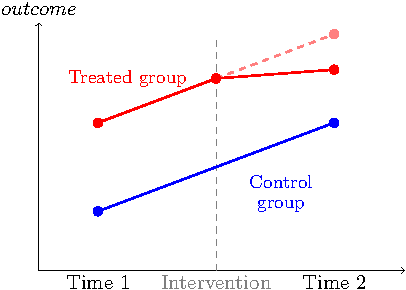
\includegraphics{hei-report_files/figure-pdf/unnamed-chunk-1-1.pdf}

To estimate the overall impact of the policy, we will use a
difference-in-differences approach (\textbf{Figure 3}), a
quasi-experimental design that compares outcomes before and after an
intervention in a treated group (one ``difference'') relative to the
same outcomes measured in a control group (the second ``difference'').
The control group trend provides the crucial ``counterfactual'' estimate
of what would have happened in the treated group had it not been
treated. By comparing each group to itself, this approach helps to
control for both measured and unmeasured fixed differences between the
treated and control groups. By measuring changes over time in outcomes
in the control group unaffected by the treatment, this approach also
controls for any unmeasured factors affecting outcome trends in both
treated and control groups. This is important since there are often many
potential factors affecting outcome trends that cannot be disentangled
from the policy if one only studies the treated group (as in a
traditional pre-post design).

\hypertarget{data-analysis}{%
\subsection{Data Analysis}\label{data-analysis}}

\hypertarget{results}{%
\subsection{Results}\label{results}}

\hypertarget{description-of-study-sample-table}{%
\subsubsection{Description of study sample
(Table)}\label{description-of-study-sample-table}}

\begin{itemize}
\tightlist
\item
  Study flowchart of participants (Figure)
\item
  Description of PM measurements (Figure)
\item
  Uptake of the policy (Sankey energy use)
\item
  Impact of `treatment assignment' on coal use
\end{itemize}

\hypertarget{aim-1}{%
\subsubsection{Aim 1}\label{aim-1}}

\begin{itemize}
\tightlist
\item
  Impact of policy on PM mass (Figure)
\item
  Table of CDEs (Central SBP, Central DBP, FeNO, Respiratory outcomes,
  inflammatory markers), mediated by indoor PM (CDEs for personal and
  outdoor in SI)
\item
  Table for multiple mediation analysis for BP
\end{itemize}

\hypertarget{aim-2-was-aim3}{%
\subsubsection{Aim 2 (was Aim3)}\label{aim-2-was-aim3}}

\begin{itemize}
\tightlist
\item
  Figure of source contributions (6 or fewer components)
\item
  Source contributions by treatment status
\item
  DiD for source contributions to PM
\end{itemize}

\hypertarget{aim-3}{%
\subsubsection{Aim 3}\label{aim-3}}

\begin{itemize}
\tightlist
\item
  Table of mediated health effects by source contribution (coal and
  biomass)
\end{itemize}

\hypertarget{discussion-and-conclusions}{%
\subsection{Discussion and
Conclusions}\label{discussion-and-conclusions}}

Other relevant results (Tables or figures in SI) - Temperature - Heating
room - Well-being

\hypertarget{implications-of-findings}{%
\subsection{Implications of Findings}\label{implications-of-findings}}

To come\ldots{}

\hypertarget{data-availability-statement}{%
\subsection{Data Availability
Statement}\label{data-availability-statement}}

To come\ldots{}

\hypertarget{acknowledgements}{%
\subsection{Acknowledgements}\label{acknowledgements}}

To come\ldots{}

\hypertarget{references}{%
\subsection{References}\label{references}}

\hypertarget{refs}{}
\begin{CSLReferences}{1}{0}
\leavevmode\vadjust pre{\hypertarget{ref-callaway2020a}{}}%
Callaway B. 2020.
\href{https://doi.org/10.1007/978-3-319-57365-6_352-1}{Difference-in-{Differences}
for {Policy Evaluation}}. In: \emph{Handbook of {Labor}, {Human
Resources} and {Population Economics}} (K.F. Zimmermann, ed). {Springer
International Publishing}:{Cham}. 1--61.

\leavevmode\vadjust pre{\hypertarget{ref-li2022}{}}%
Li X, Baumgartner J, Barrington-Leigh C, Harper S, Robinson B, Shen G,
et al. 2022a. Socioeconomic and {Demographic Associations} with
{Wintertime Air Pollution Exposures} at {Household}, {Community}, and
{District Scales} in {Rural Beijing}, {China}. Environmental Science \&
Technology 56:8308--8318;
doi:\href{https://doi.org/10.1021/acs.est.1c07402}{10.1021/acs.est.1c07402}.

\leavevmode\vadjust pre{\hypertarget{ref-li2022a}{}}%
Li X, Baumgartner J, Harper S, Zhang X, Sternbach T, Barrington-Leigh C,
et al. 2022b. Field measurements of indoor and community air quality in
rural {Beijing} before, during, and after the {COVID-19} lockdown.
Indoor Air 32:e13095;
doi:\href{https://doi.org/10.1111/ina.13095}{10.1111/ina.13095}.

\leavevmode\vadjust pre{\hypertarget{ref-sternbach2022}{}}%
Sternbach TJ, Harper S, Li X, Zhang X, Carter E, Zhang Y, et al. 2022.
Effects of indoor and outdoor temperatures on blood pressure and central
hemodynamics in a wintertime longitudinal study of {Chinese} adults.
Journal of Hypertension 40:1950--1959;
doi:\href{https://doi.org/10.1097/HJH.0000000000003198}{10.1097/HJH.0000000000003198}.

\end{CSLReferences}

\hypertarget{appendices}{%
\subsection{Appendices}\label{appendices}}

\hypertarget{about-the-authors}{%
\subsection{About the authors}\label{about-the-authors}}

\hypertarget{other-publications}{%
\subsection{Other publications}\label{other-publications}}

Other papers that have been published.(Li et al. 2022a; Li et al. 2022b;
Sternbach et al. 2022)



\end{document}
